\newpage
{\color{gray}\hrule}
\begin{center}
\section{Comparison of Solutions}
\bigskip
\end{center}
{\color{gray}\hrule}
\begin{multicols}{2}

\begin{enumerate}
    \item The response of the series RL circuit to a square wave input was computed using both numerical and analytical methods. 
    \item The numerical solution was obtained by solving the differential equation using the Trapezoidal Rule, while the analytical solution was derived using the Fourier series representation of the input signal.
    \item Upon plotting the results from both methods, it was observed that the numerical and analytical solutions produced identical waveforms. 
\end{enumerate}
\begin{figure}[H]
  \centering
  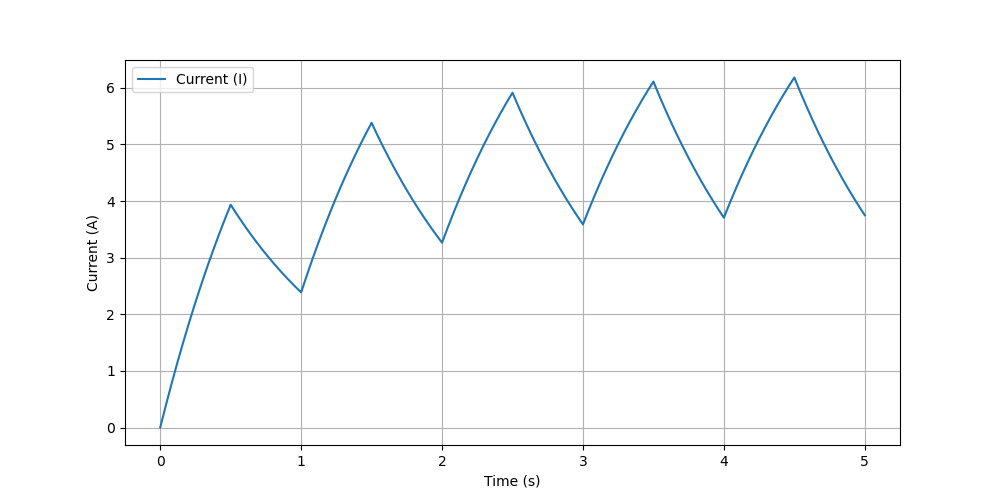
\includegraphics[width=\columnwidth]{sections/4_og.png}
  \caption{Response Obtained via Numerical Method}
\end{figure}
\begin{figure}[H]
  \centering
  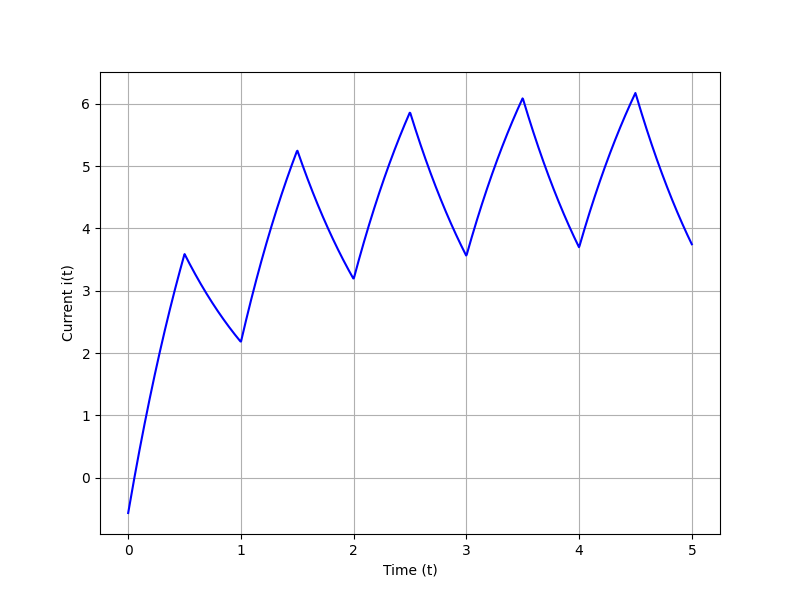
\includegraphics[width=\columnwidth]{sections/5_Analytical.png}
  \caption{Response Obtained via Analytical Method}
\end{figure}
This indicates that the numerical integration method accurately approximates the theoretical response of the circuit.

\end{multicols}
